\subsection{平方根形状的有界自然梯度与显式动力学}

由式~\eqref{eq:proximal-natural-velocity}，$\|v_\kappa\|_F^2=\Var_q(\rho^\kappa)/\kappa^2$。当 $0<\kappa\le1/2$，$2\kappa\le1$，Jensen 不等式给出 $\E_q\rho^{2\kappa}\le(\E_q\rho)^{2\kappa}=1$，于是
\begin{equation}
 \|v_\kappa\|_F^2\le\frac{1-a_\kappa^2}{\kappa^2}\le\frac1{\kappa^2}.
 \label{eq:proximal-natural-speed-bound}
\end{equation}
该界对任意完整支持的 $q,T$ 成立，不需要给 teacher 或 student 指定统一概率下界。对于 $\kappa>1/2$，取 $q=(\varepsilon,1-\varepsilon)$、$T=(c,1-c)$，$0<c<1$ 固定，则
\begin{equation}
 \Var_q(\rho^\kappa)
 =\varepsilon(1-\varepsilon)
 \left[(c/\varepsilon)^\kappa-((1-c)/(1-\varepsilon))^\kappa\right]^2
 \sim c^{2\kappa}\varepsilon^{1-2\kappa}\longrightarrow\infty.
\end{equation}
几何端点 $\kappa=0$ 也没有统一界：固定 $q=(1/4,3/4)$、令 $T=(\varepsilon,1-\varepsilon)$，$\Var_q\log(T/q)$ 随 $\varepsilon\to0$ 发散。故 $0<\kappa\le1/2$ 是这个自然梯度族具有统一 Fisher 速度界的区间。确定性的 Fisher 速度与随机参数梯度方差是不同对象，不能把这个结论直接写成完整训练梯度的方差定理。

在平方根点 $\kappa=1/2$，$a=\sum\sqrt{qT}$，并有 $\E_q\rho=1$，因此
\begin{equation}
 \|v_{1/2}\|_F^2=4(1-a^2)\le4,\qquad
 D_{1/2}(T\Vert q)=4(1-a).
\end{equation}
由 Lyapunov 等式，连续流满足
\begin{equation}
 \frac{da}{dt}=1-a^2,
 \qquad a(t)=\tanh(t+\operatorname{artanh}a(0)),\quad q\ne T.
 \label{eq:proximal-hellinger-flow}
\end{equation}
证明是 $dD_{1/2}/dt=-4\,da/dt=-4(1-a^2)$，然后积分 $da/(1-a^2)=dt$。$q=T$ 时 $a=1$ 且流恒定。进一步，$D'=-(1+a)D$，由于 $0<a\le1$，有
\begin{equation}
 D(0)e^{-2t}\le D(t)\le D(0)e^{-t}.
\end{equation}
若写 $a=\cos\vartheta$，则 $d\vartheta/dt=-\sin\vartheta$。平方根形状既有球面解释，也有显式 teacher 接近度和有界 Fisher 速度。这使它成为一个有数学依据的候选点，尚不能据此断言其训练性能优于其他形状。

\begin{figure}[htbp]
 \centering
 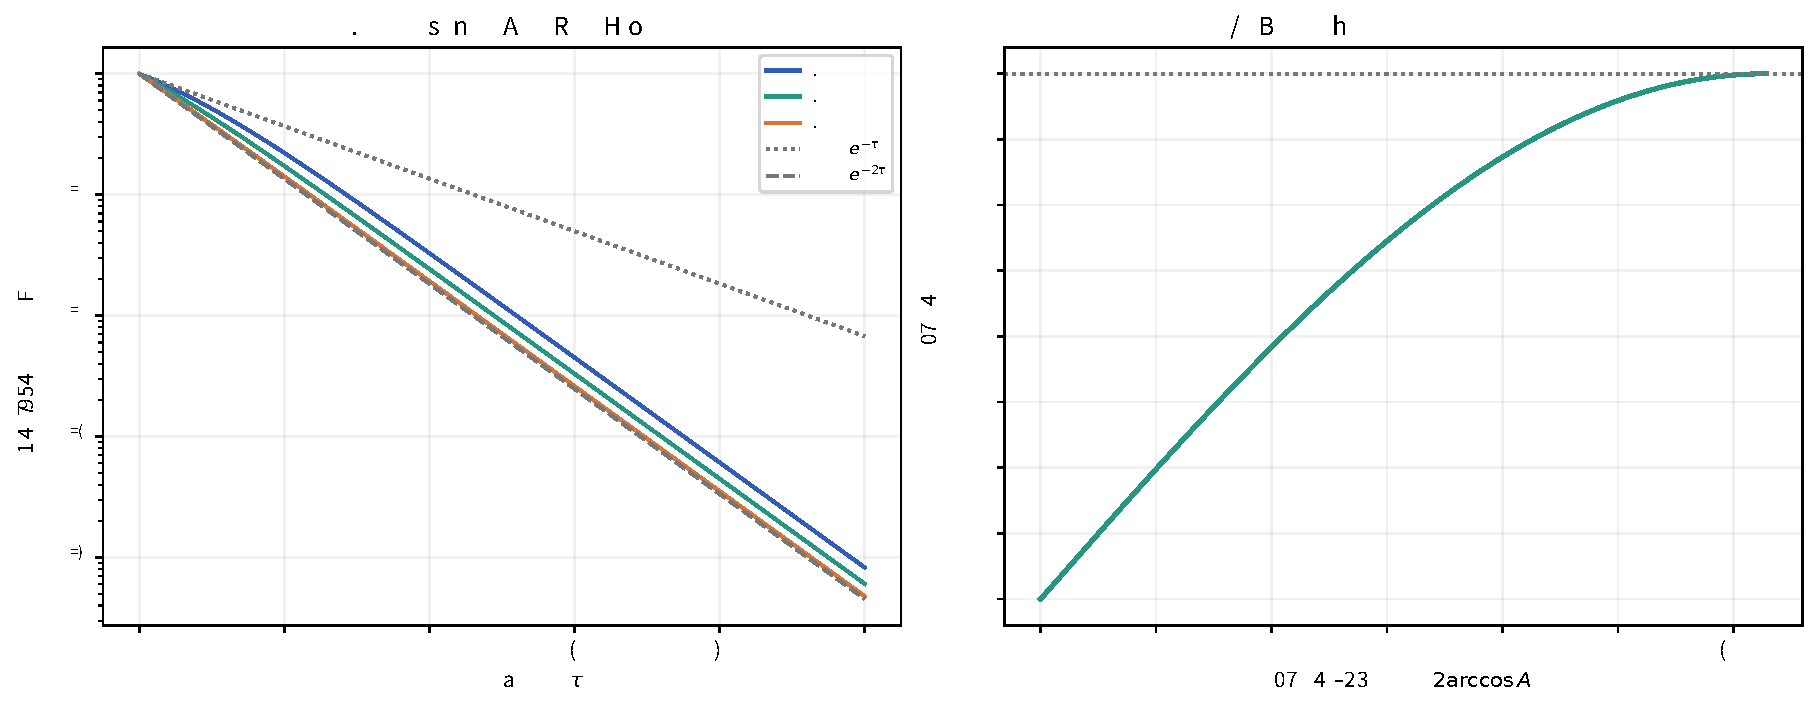
\includegraphics[width=\textwidth]{../../results/proximal-family-geometry/hellinger-flow.pdf}
 \caption{平方根形状的连续动力学。左图由 $a(t)=\tanh(t+\operatorname{artanh}a(0))$ 精确生成，归一化散度位于两个指数包络之间；右图将 Fisher 速度写成到 teacher 的 Fisher--Rao 距离函数，展示统一上界 2。}
\end{figure}
